\documentclass[11pt]{amsart}
\usepackage{geometry}                % See geometry.pdf to learn the layout options. There are lots.
\geometry{letterpaper}                   % ... or a4paper or a5paper or ... 
%\geometry{landscape}                % Activate for for rotated page geometry
%\usepackage[parfill]{parskip}    % Activate to begin paragraphs with an empty line rather than an indent
\usepackage{graphicx}
\usepackage{amssymb}
\usepackage{epstopdf}
\usepackage{enumerate}
\DeclareGraphicsRule{.tif}{png}{.png}{`convert #1 `dirname #1`/`basename #1 .tif`.png}
\setlength{\parindent}{0in} % no paragraph indent

\usepackage{fancyhdr}
\pagestyle{fancy}
\lhead{\footnotesize \parbox{11cm}{The Effect of the NSA Leaks on Tech Stock Volatility} }
\rhead{\footnotesize \parbox{5cm}{Max Scheiber and Ruslan Zagatskiy} }

\title{The Effect of the NSA Leaks on Tech Stock Volatility - Max Scheiber and Ruslan Zagatskiy}
\date{12.16.2013}

\begin{document}
\maketitle
\section{Abstract}
The NSA scandal of the summer of 2013 changed the way that many Americans viewed the relationship between government and citizens. However, these changes were not strongly reflected in either short-term or long-run technology stock volatility . At most, one of ex-employee Edward Snowden's early leaks caused an isolated spike in volatility. Overall, there were no other significant changes in return volatility or trading volume in securities of companies that the NSA claimed to have data-sharing agreements with. \\

\section{Introduction}
On June 6th, 2013, Edward Snowden revealed through the British newspaper, \textit{The Guardian}, that the National Security Agency (NSA) can easily extract personal customer data from America's largest tech companies, spanning from email to audio chats. More NSA leaks were released throughout summer 2013. These events fundamentally changed the socioeconomic and political climates of the United States of America. However, did these leaks change the volatility of relevant tech stocks in either the short term or long run? That is, were citizens personal reactions to the NSA leaks reflected in the securities market? \\

Examining the effect of these leaks on the stock market requires an event-driven approach. A standard way to consider specific date ranges quantitatively is to create a dummy indicator variables for the dates in question. Statisticians can then use these variables as an input to any statistical model, such as a linear regression or more complex time series model. As Savickas wrote in 2003, \\

\textit{I use a GARCH(1,1) model with dummy variables to evaluate a simple test statistic that accounts for the stochastic behavior of volatility during both event and nonevent periods. The test does not require the volatility effect to be the same across firms in the sample. The test is easy to implement but has substantially higher rejection rates of a false null hypothesis than do the previous tests.} \\

A GARCH(1,1) tests for heteroskedasticity in the variance of a series - in other words, whether volatility is constant throughout a period. If the coefficients for a fitted GARCH(1,1) are significant, we can infer that there were periods of volatility spikes/volatility clustering in the series. A large portion of our analysis uses a very similar model. It is important to note is that while it's easy to show results statistically, it is difficult to apply these to show causation. There will always be some room for interpretation with projects based on more qualitative events like the NSA leaks. \\

We obtained consolidated trade data from Wharton Research Data Services (WRDS) for Google (GOOG), Apple (AAPL), Microsoft (MSFT), and Facebook (FB) for the January 1st, 2013 through July 31st, 2013. These consolidated datasets contain average execution prices and total shares traded volume a few times each second. We chose these stocks because they were the ones  \textit{specifically} identified in the NSA's leaked slide deck. \\

To make data analysis more manageable, we converted this data into hourly buckets from 9am to 3pm, inclusive. We did this by taking the average execution price over each bucket, equally weighted within the bucket. We performed similar consolidation for the trade volume data. In the end, we had seven points of data per day. \\

We then created a basket of tech stocks by taking the equal-weighted average of the four above stocks. This strategy allows us to enhance our signal-to-noise ratio; this basket would minimize spikes in trade volume or volatility of, say, one company's earnings report, while confirming sector-wide trends. Significant effects that affected all four companies, like the NSA leaks, would be highlighted, while individual shocks would be mitigated. We then computed the percent returns from the basket prices. \\

We used two approaches to approximate the volatility of our basket returns. First, we considered squared returns. Since the returns were centered on zero, squaring them is equivalent to finding their variance. Second, we constructed a scale-independent moving volatility.  For this approach, we measure the volatility of a given bucket by considering the volatility of the pervious 30 buckets. Given that there are seven buckets per day, we see our volatility measure cover a duration of just over four days. All analysis in this paper is performed with both measures. \\

\section{Methods}
We explored three main dates. Snowden's original leaks happened on \textbf{June 6th, 2013}. \textit{The Guardian} released a second set of leaks on \textbf{June 20th}, and they published a video interview with Snowden on \textbf{July 8th}. We consulted multiple sources and found that these were the most prominent and well-publicized dates of NSA leaks.  \\

We first examined our volatility for the entire data set, noting that there were significant spikes throughout and the June/July looked significantly volatile. We then ran a $GARCH(1,1)$ on returns over our entire time frame, which confirmed the heteroskedasticity we would expect in the variance of the series. This makes intuitive sense: the stock market probably is likely to have several periods of abnormal trading over a seven-month span. If anything, we would have been surprised to find homoskedasticity. \\

\centerline{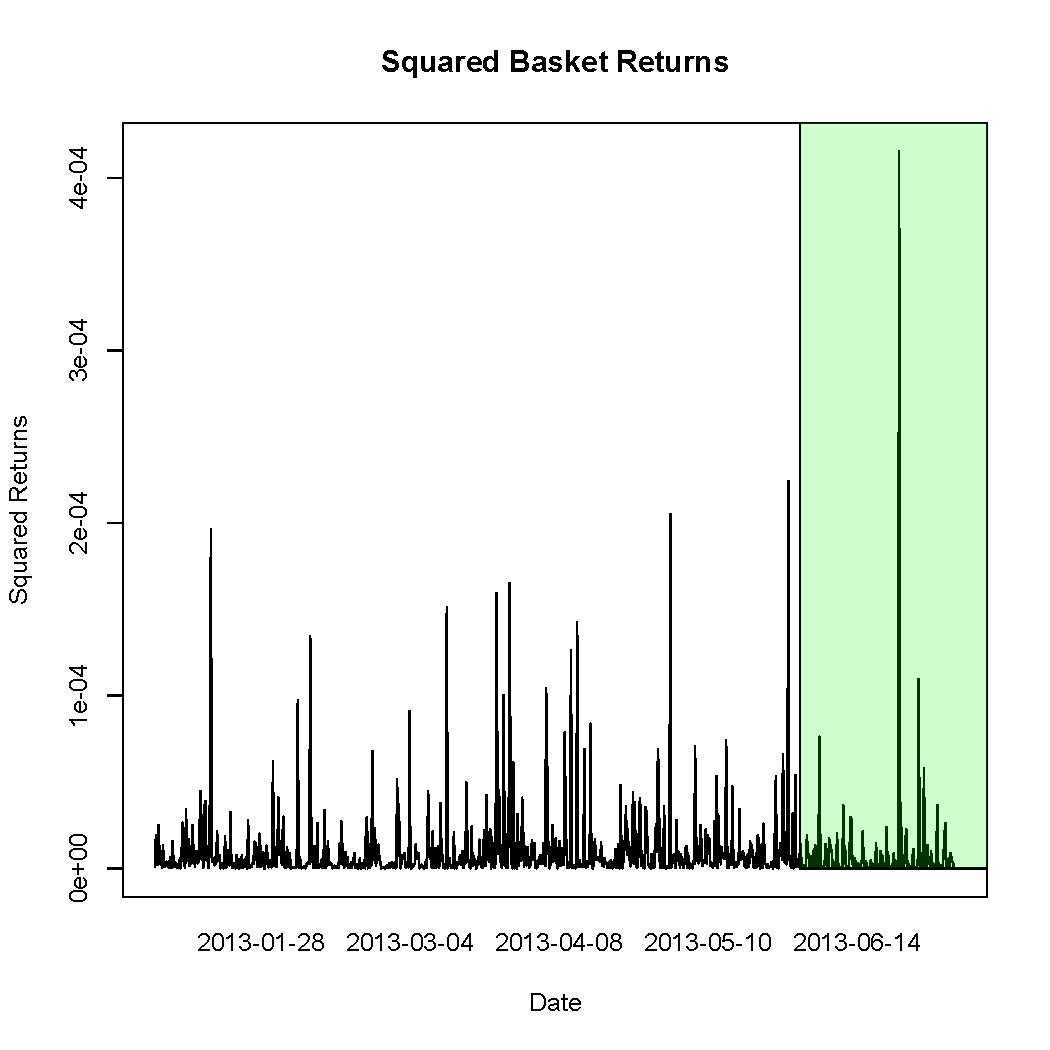
\includegraphics[scale=0.5]{basket_sq_returns_12_08.pdf}}

We next examine the month of June, our first month of interest. June itself exhibits heteroskedasticity in the variance of its returns, confirmed by another $GARCH(1,1)$.  To determine whether any of the volatility spikes had a notable effect on June volatility, we plotted the cumulative sum of standardized recursive residuals of a volatility regression. The CUSUM functions breaks the 95\% error bands towards the end of June confirming that there is an impact large enough to suggest a structural change in the data.\\

\centerline{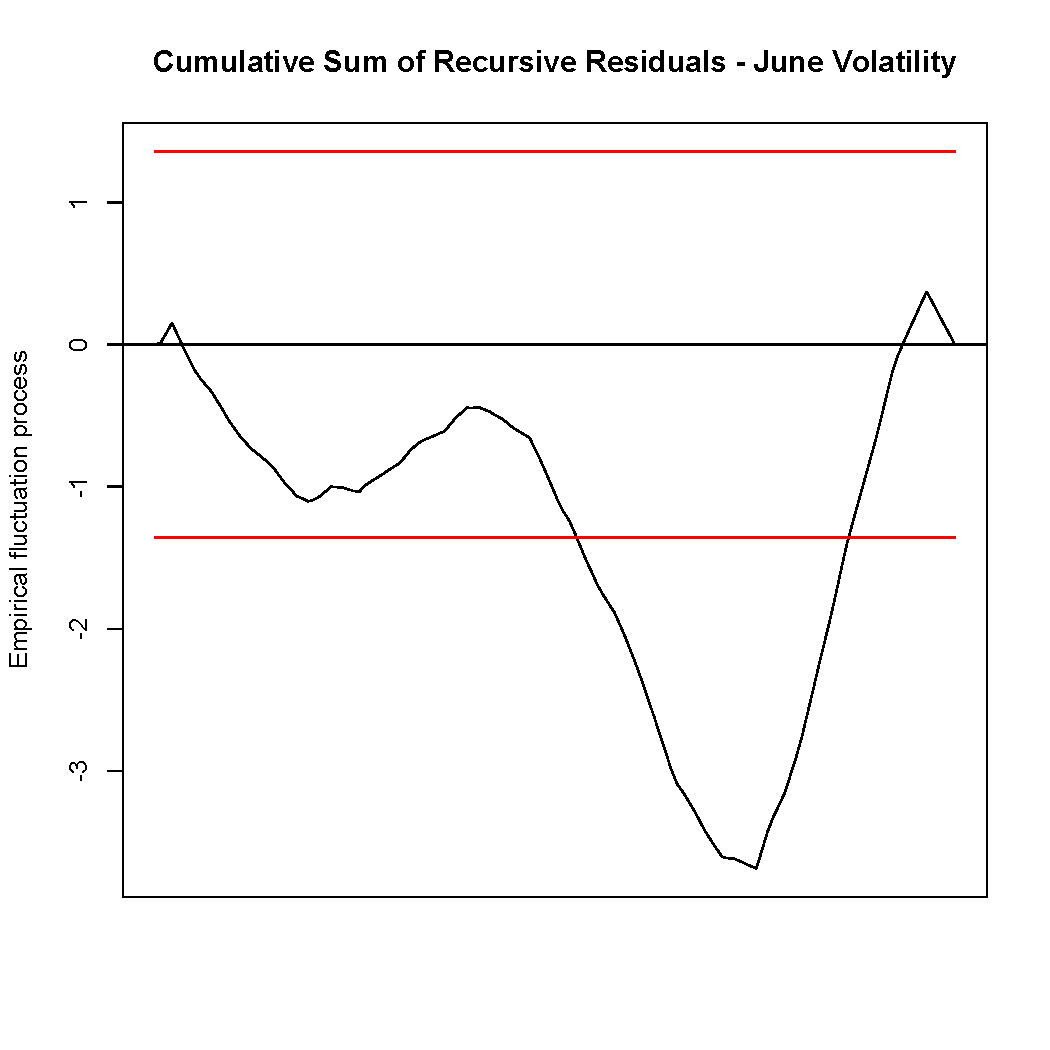
\includegraphics[scale=0.45]{june_cusum.pdf}}

We next fit an OLS regression with indicator variables for June 6-7 and June 20-21, two dates of interest. Only the change in volatility during June 20-21 was statistically significant. We considered whether this effect was only short-term by exploring the possibility of medium or long-run regime change post-June 20th. In fact, the spike in volatility is only significant in the short term (June), not medium term (June-July) or long term (January-July). \\

We continued our analysis for June by considering trade volume, a natural partner for volatility. Darrat, Zhong, and Cheng notes that "[there is] bi-directional causality between volume and volatility."  Similar to volatility, June trade volume is heteroskedastic (again confirmed by the $GARCH(1,1)$) and significant on the June 20-21 date range. \\

Next, we perform similar analysis for the month of July. We see a huge spike in volatility centered  around July 20th, but this doesn't correspond with any NSA news. It's likely from quarterly earnings reports - GOOG and MSFT on the 18th, AAPL and FB on the 24th. This highlights the causation problem mentioned above.The same event-driven models used in previous section confirm the statistical significance of a July 20th effect, but this result is not interesting for our analysis. Unfortunately, a regression with the July 8th range indicator is not significant. Similar to June, these results are mirrored for July trade volume. \\

\centerline{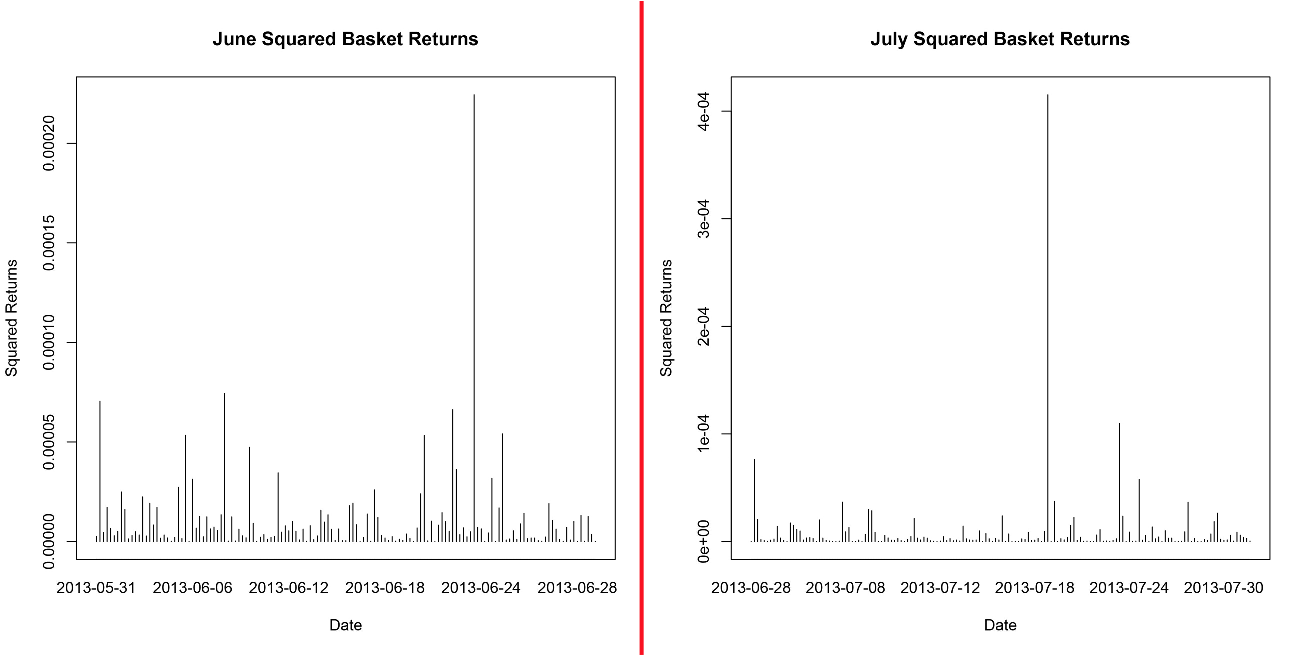
\includegraphics[scale=0.7]{june+july_squared_ret.pdf}}

To get a better sense of the American economic climate at the time, we looked into other large events that would have affected overall stock market. Around June 20th, the only large event was the NSA leak. The Federal Reserve had made an announcement regarding its bond buyback program, but we felt that was minor in comparison to other Fed announcements throughout 2013. It is worth noting that the comparison was that June 20th had one of the three largest spikes in volatility throughout all of 2013 for the VIX, the S\&P 500's exchange-traded fund.

\section{Conclusions}
Event-driven analysis is hard to draw conclusions from because it is difficult to untangle correlation from causation. While the statistical analysis we performed was sound, the qualitative analysis performed is not rock-solid. It is hard to avoid confirmation bias when performing qualitative event analysis. We specifically set our dates of concern before even looking at data to avoid being biased in that way, but confirmation bias may have crept in while investigating whether the June 20th volatility spike was caused by something other than the NSA leak. \\

If the NSA leaks have changed how we view the world, the market doesn't really reflect that. There was increased volatility in response to one of the leaks, which may have just been some large institutional investor unloading shares. Moreover, this volatility only persisted for a couple of days. Given that our qualitative analysis is sound, \textbf{the NSA leaks affected short-term volatility in one instance but had no long-term effect whatsoever.} Moreover, any change in volatility that \textit{did} happen affected the entire market, not just tech stocks. \\

\newpage
\section{Appendix}

\subsection{Google analysis}
Before performing analysis on the basket of stocks, we performed some basic analysis of Google's returns. \\

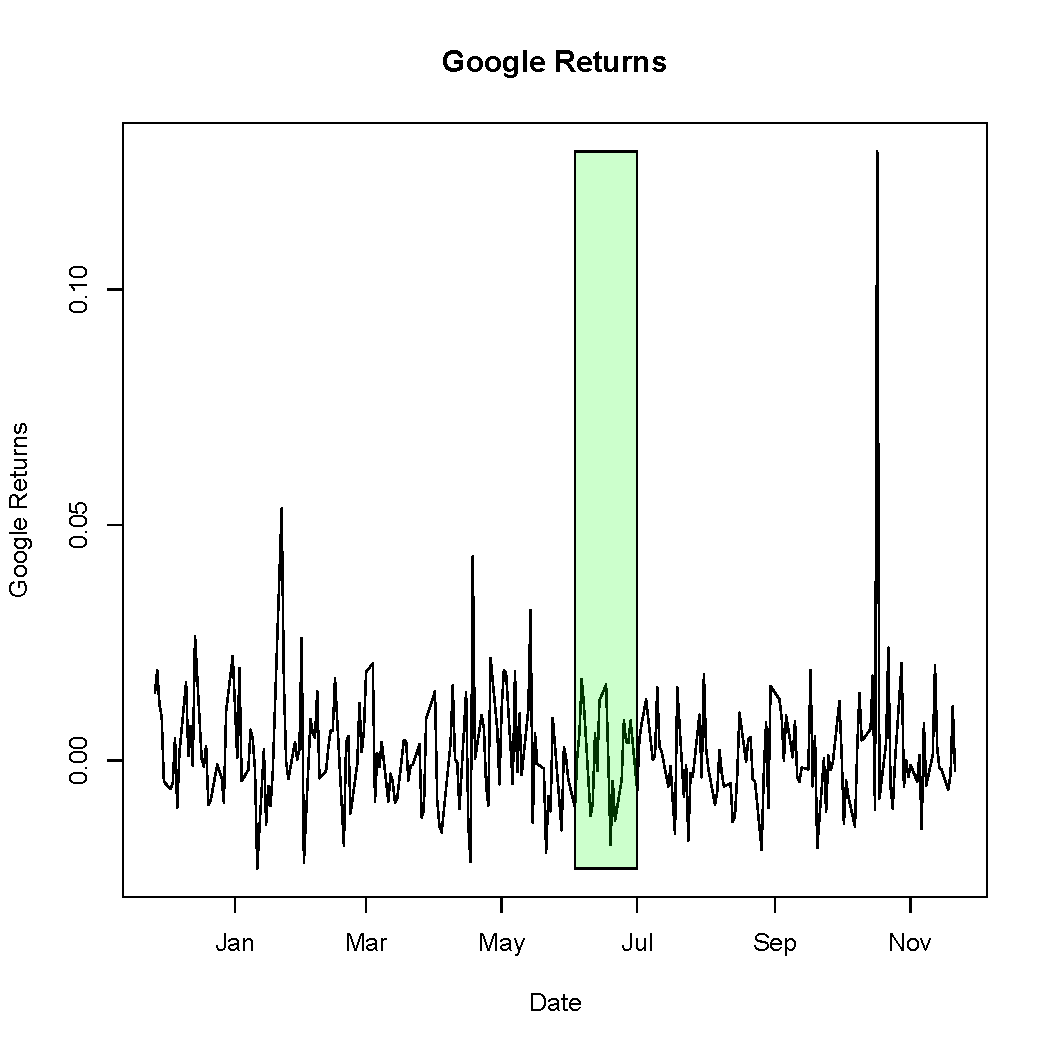
\includegraphics[scale=0.4]{goog_returns_11_25.pdf} \\

Immediately, we can see that Google did not really have any outliers in its return over the summer. Its main spikes seem to come from its earning reports, implying that the market did not judge the NSA scandals to really affect Google. \\

We next look at Google's hourly volatility throughout June, which is when the majority of the NSA leaks happened. It initially seems obvious via eyeballing that Google's volatility spiked on June 6th (the date of \textit{The Guardian}'s first leak) and June 20th (the date of \textit{The Guardian}'s second leak). \\

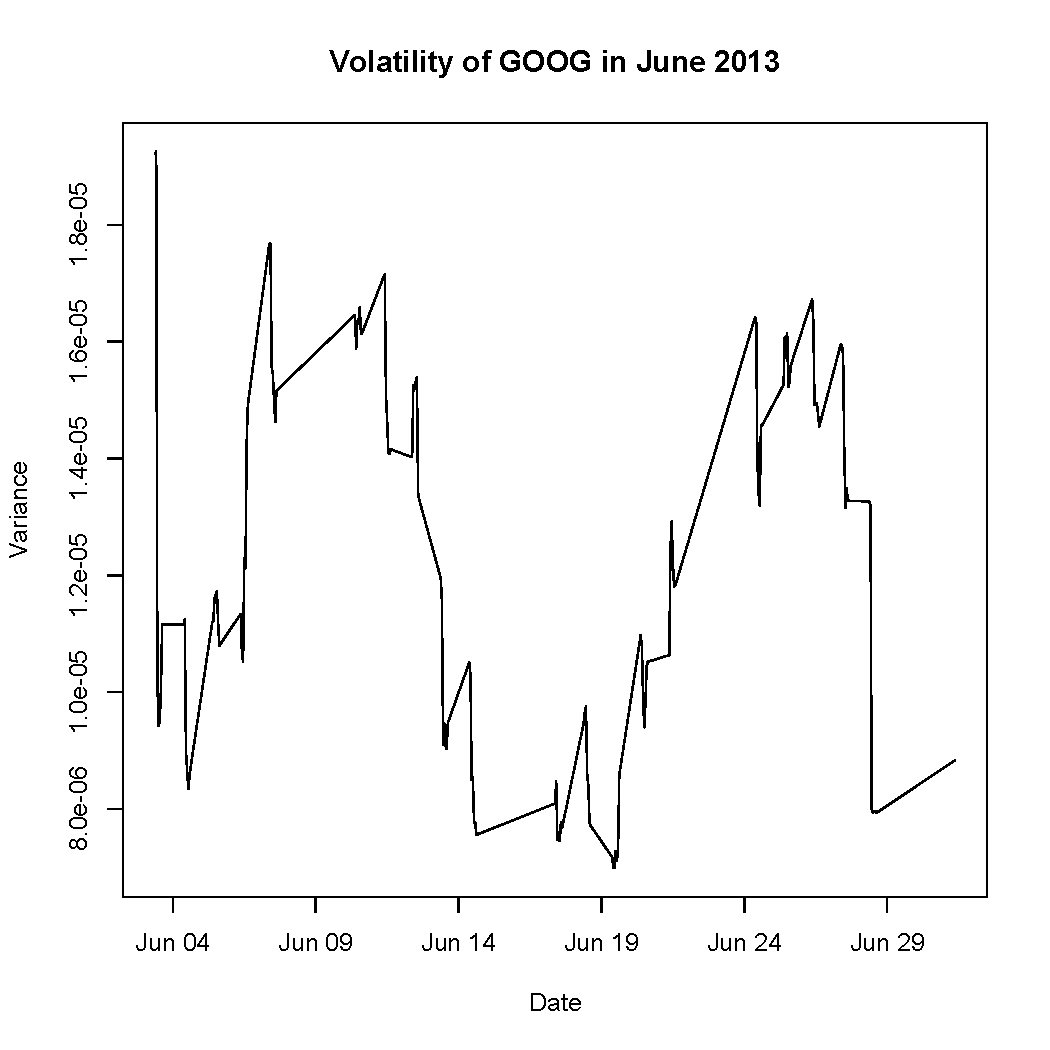
\includegraphics[scale=0.4]{goog_vol_zoom_11_25.pdf} \\

However, in context, these spikes are extremely minimal. Let us, for example, plot volatility throughout 2013. \\

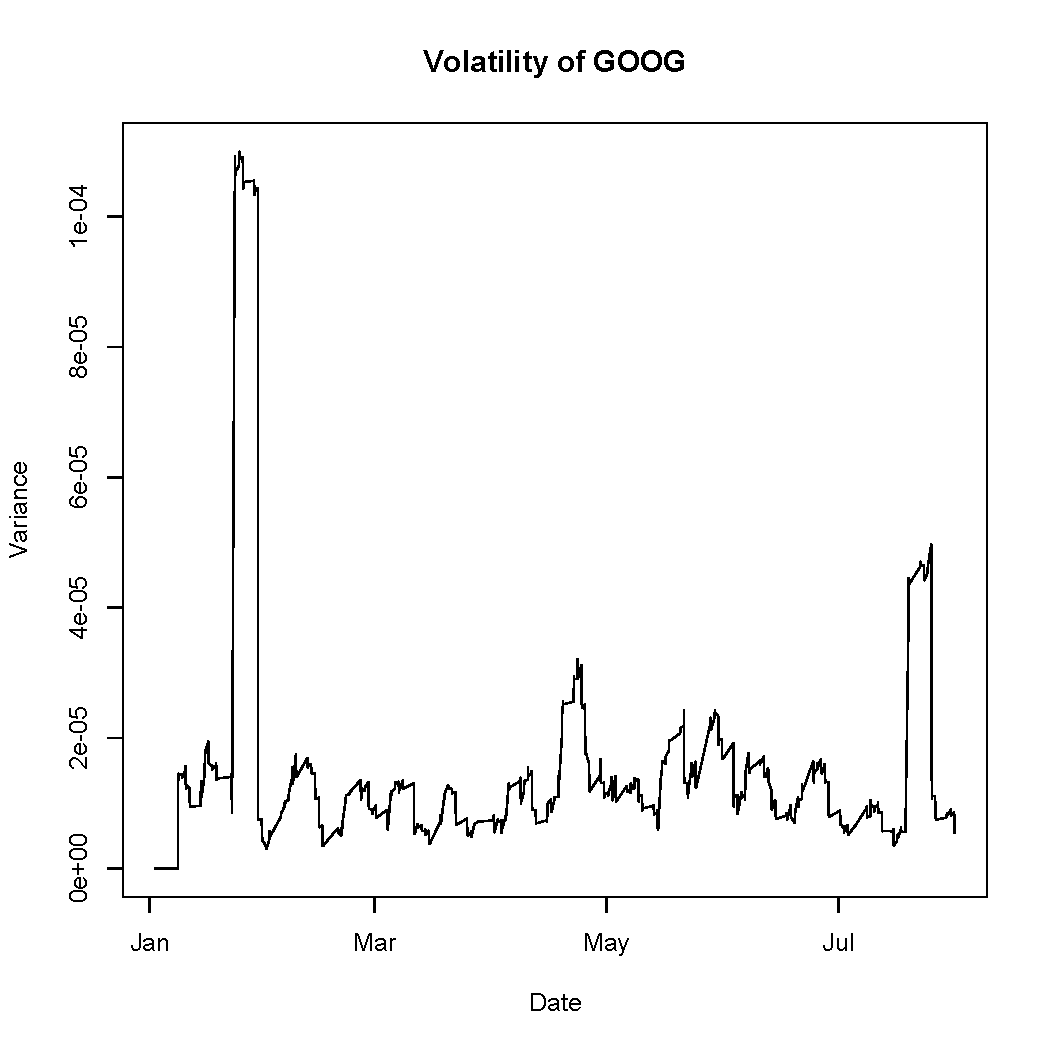
\includegraphics[scale=0.4]{goog_vol_11_25.pdf} \\

Any June spikes that could be related to the NSA do not look very significant in the context of Google's volatility throughout the year. While it is ostensible that these small June spikes may indeed have occurred as a result of the NSA scandal, this seems to be an early indicator that our hypothesis may not hold.

\newpage
\subsection{Tech sector basket analysis - full data set}
For further confirmation, we now look at the full tech sector basket as discussed in section 2. \\

To check for any sort of heteroskedasticity, we plot squared returns of the basket. Note that while we also
applied our moving volatility model to basket data, the plot of squared returns provides a simpler visual 
analysis that leads to the same conclusions.\\

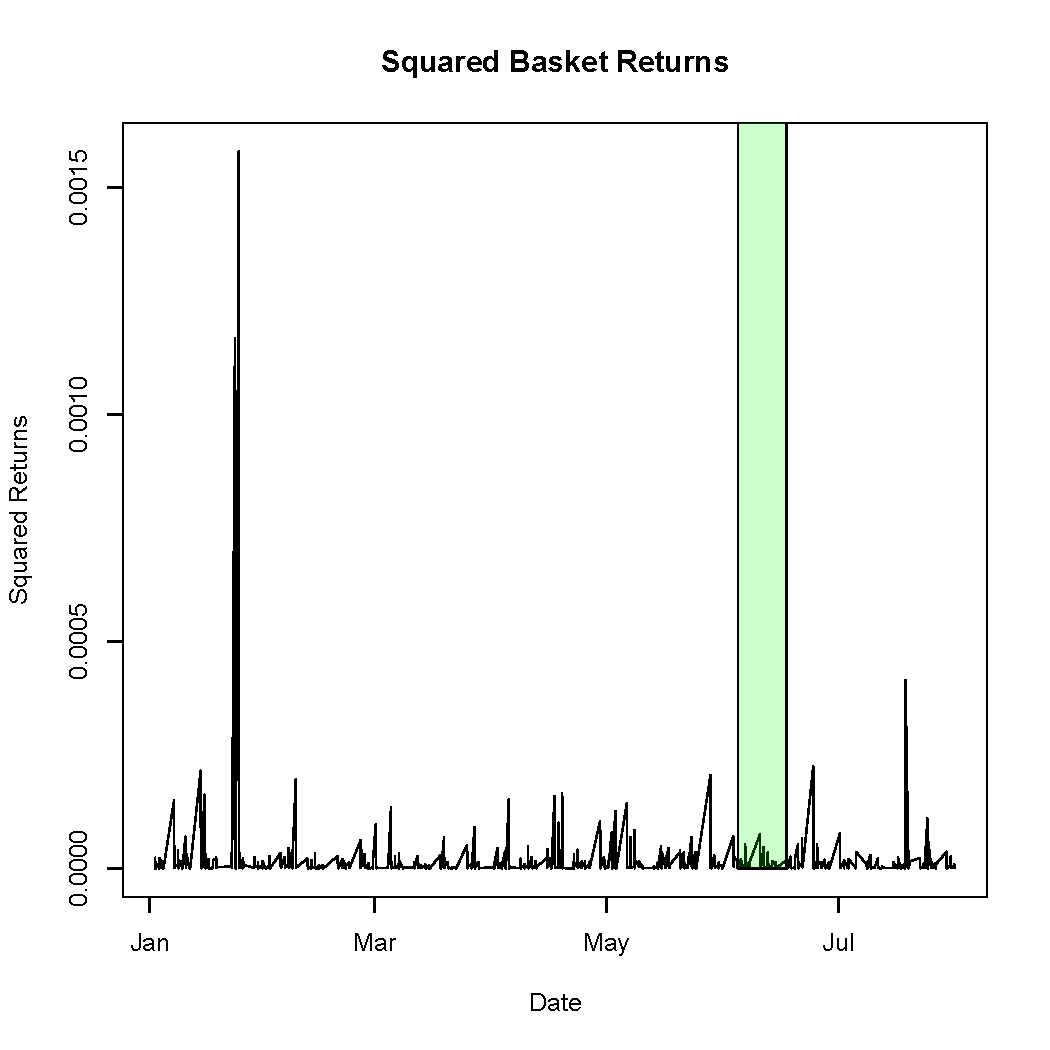
\includegraphics[scale=0.4]{basket_sq_returns_11_25.pdf} \\

\newpage
While the basket's 2013 squared returns have some unusual spikes,  it looks generally stable. More rigorously, we considered an ARCH(1) model for the basket's returns. The model's first coefficient is statistically insignificant, implying homoskedasticity. Of course, testing just an ARCH(1) is not sufficient. Next we look at an ARCH(8), where we find that the 6th and 7th lags are significant. Finally, we consider a GARCH(1,1), which is essentially equivalent to an 
infinte order ARCH. The significance of both the ARCH(alpha1) and GARCH(beta1) terms confirms heteroskedasticty
in the basket return variance.  \\



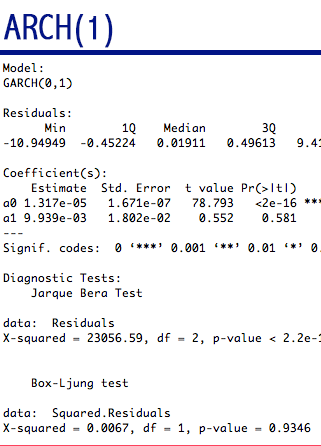
\includegraphics[scale=0.5]{arch1_basket_11_25.png} \\
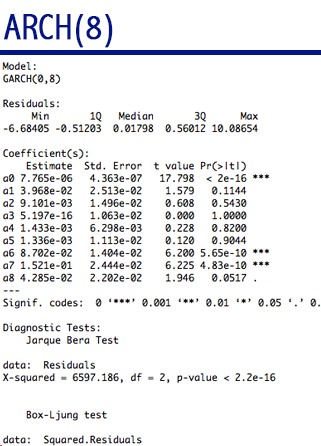
\includegraphics[scale=0.5]{arch8_basket_12_2.png} \\
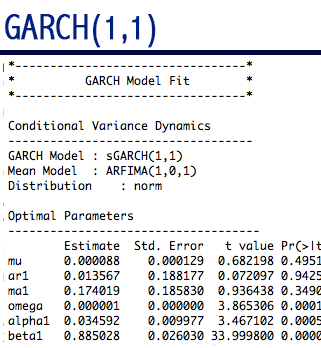
\includegraphics[scale=0.5]{garch11_basket_12_2.png} \\

\newpage
\subsection{June indicator variables}

The discovery above is unsurprsing - heteroskedastic variance is a common feature of financial returns. A more interesting question is whether the NSA leaks, independent of other events, impacted volatility. \\

One approach is to regress using an indicator variable. We set an indicator variable to be true for all buckets on June 6th, the day of the first NSA leak, and we set another indicator variable to be true for all buckets on June 20th, the day of a large second NSA leak. We test the significance of these indicators first for our full data set and find that neither have t-Statistics large enough to reject the null that they have no impact. \\

The section above considers long-run impact of the NSA leaks on the volatiltiy of our tech basket. However, it is
also worth considering short-run volatility changes centered around the time of the leaks. We first consider the month of June since that is when the leaks began. A plot of squared returns suggests that there is some increased volatiltiy towards the end of June, particularly around June 21st (our model's volatility is lagged by about 3 days). This is confirmed by a GARCH(1,1), which has significant coefficients for lagged variance and lagged squared error terms. \\

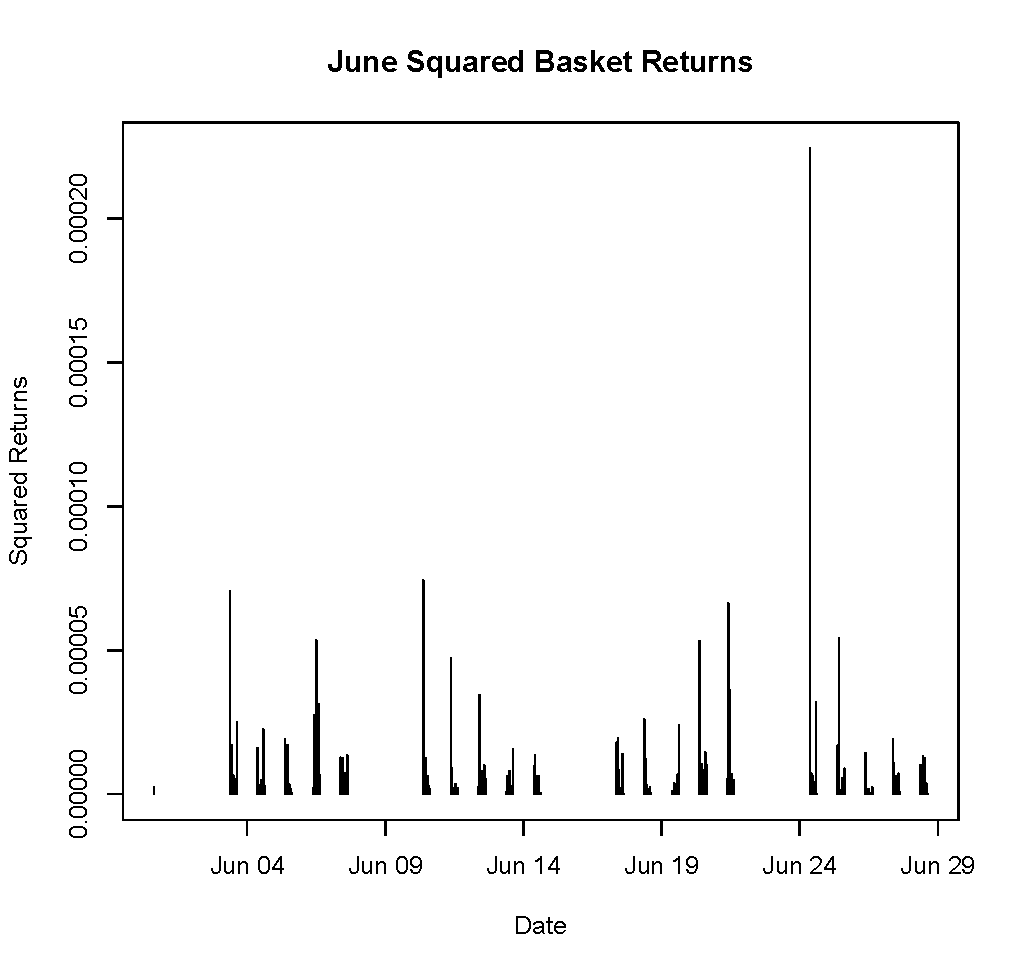
\includegraphics[scale=0.6]{june_squared_basket_ret.pdf} \\

\newpage
The result of these regressions is that only the June 20th leak is statistically significant for June volatility. The June 6th indicator does not have significant explanatory power for volatility in June or in all of 2013. It is arguable that \textit{The Guardian}'s second leak did spur more volatility in the market, but this washes out in the long run due to other similar events that affect the tech sector. There are a variety of possible explanations for the significance of June 20th versus the  null effect of June 6th, but these are purely speculative. \\

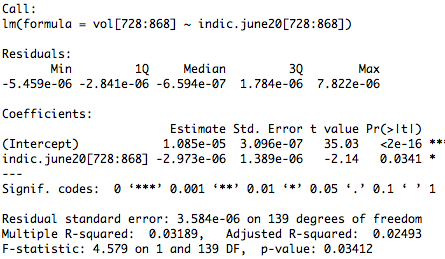
\includegraphics[scale=0.6]{june_20_june_11_25.png} \\

\newpage
It is worth highlighting that June is not a particularly volatile month. This raises the question of whether these spikes were truly caused by the NSA leak or are just a product of the basket's natural long-run volatility; June's volatiltiy looks fairly tame in the grand scheme of things. This is illustrated in the plot below, which compares June (black) with three random months. If anything, June's volatility is lower than the random months. What this is suggests is that \textit(even if) the NSA leak caused a surge in volatility, the change was so small that it is hardly worth mentioning. \\

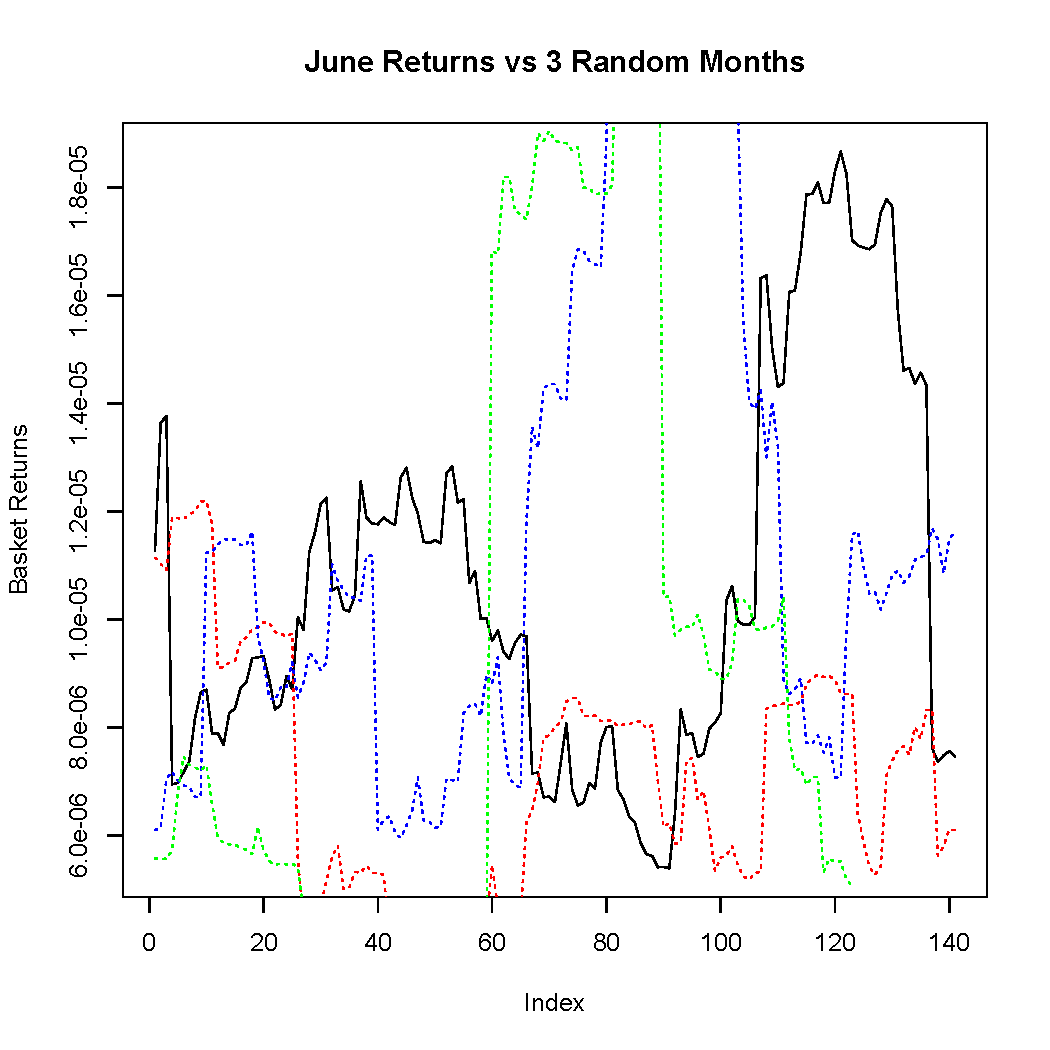
\includegraphics[scale=0.7]{june_3_months.pdf} \\

\newpage
\subsection{July indicator variables}
Next, we will consider July. A plot of squared July returns suggests a volatility spike sometime around July 18th. This is confirmed by a basic ARCH(1) model. \\

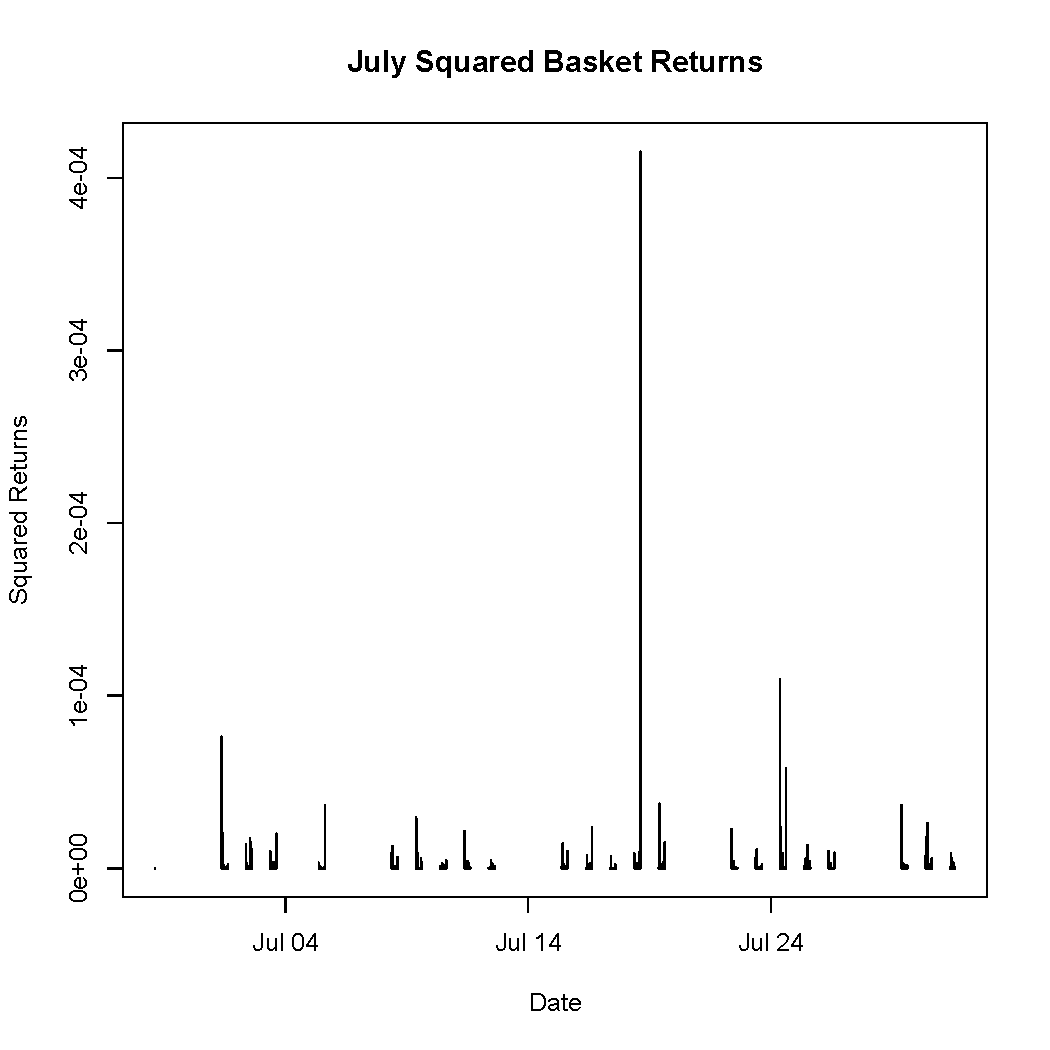
\includegraphics[scale=0.6]{july_squared_basket_ret.pdf} \\

While this initially seeming promising, it is worth noting that all of our companies had earnings reports at approximately those dates. Historically, company earnings reports have a large impact on volatility; investors are eager to adjust their portfolios based on the release of new public information. The plot below shows the squared returns of our four companies (colored) and the basket squared returns. The spikes in the company volatities are likely casued by their respective earnings releases; these combine to see the volatility spike in the basket. \\

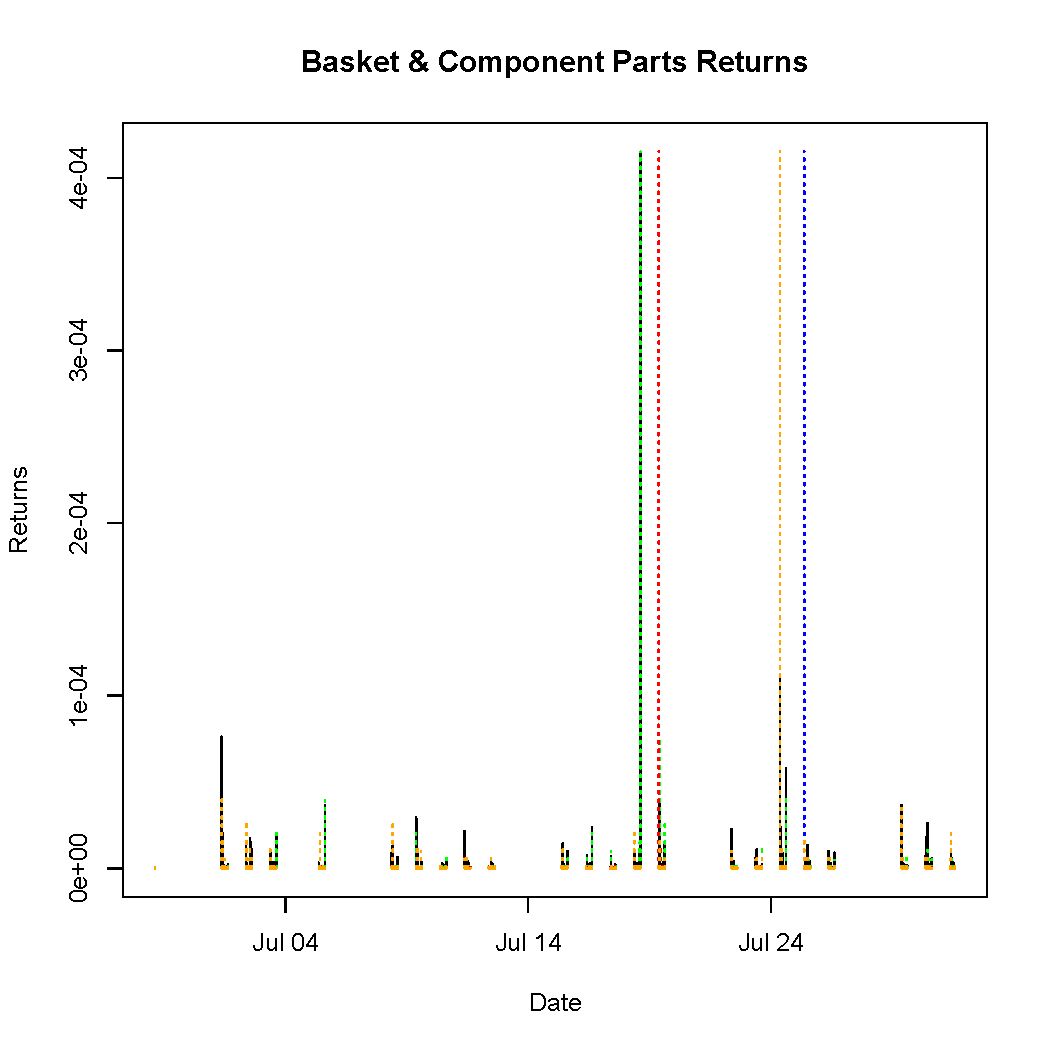
\includegraphics[scale=0.5]{july_earnings.pdf} \\

Finally, we can note that July volatility was not particularly large relative to other months in 2013. A plot comparing July volatility to the volatility in 3 random months is shown below. The results here are similar to those of June: even if the NSA leaks did have an effect, it was so small that it was hardly worth noticing. \\

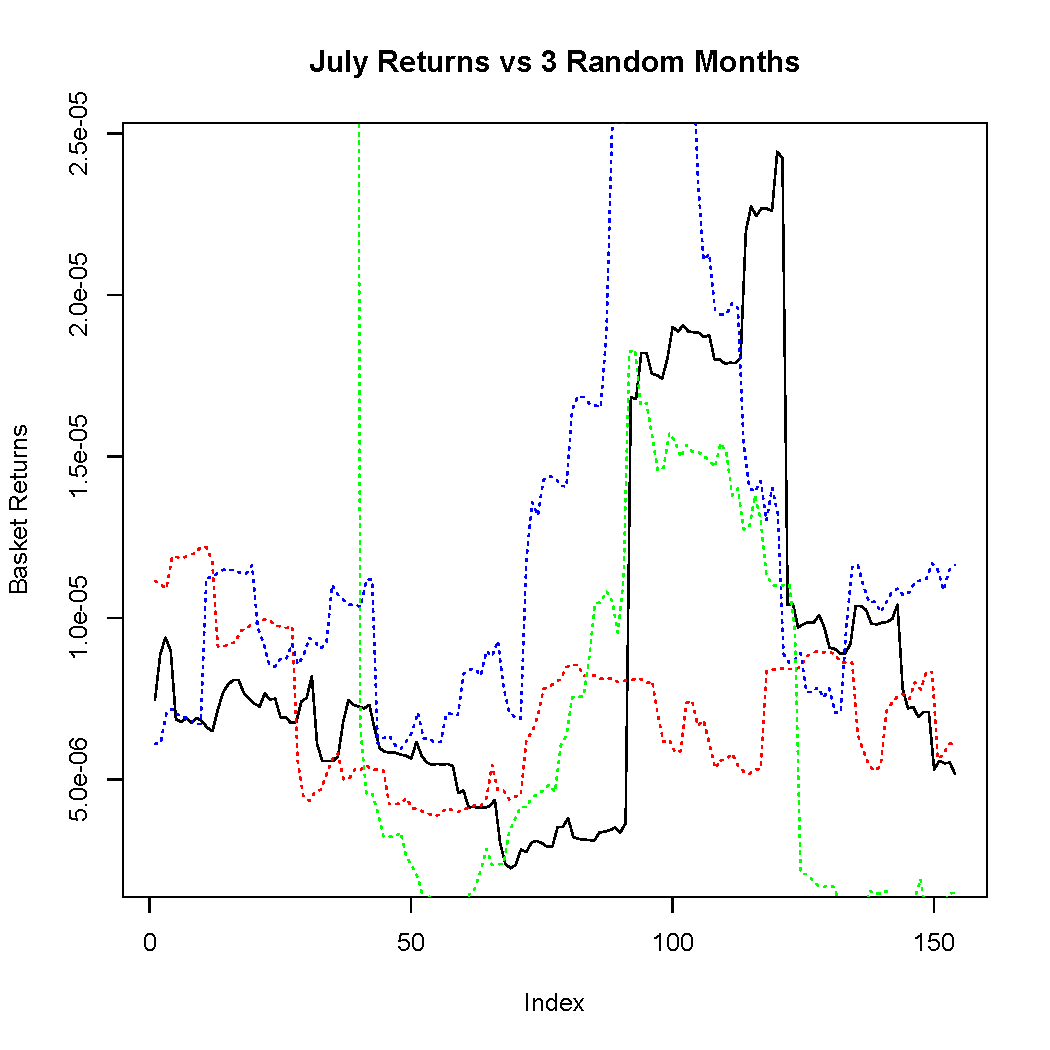
\includegraphics[scale=0.5]{july_3_months.pdf} \\

\newpage
\subsection{Volume}

So far, our volatility analysis hasn't worked out very well - we have just one probable date: June 20th. Now, let's look at another measure of market interest - volume.  \\

Let's take a look at volume for our entire data set, with June - end of July highlighted. Overall, we're seeing a lot of fluctuations in volume across the board, but our window from June - end of July looks particularly volatile. 

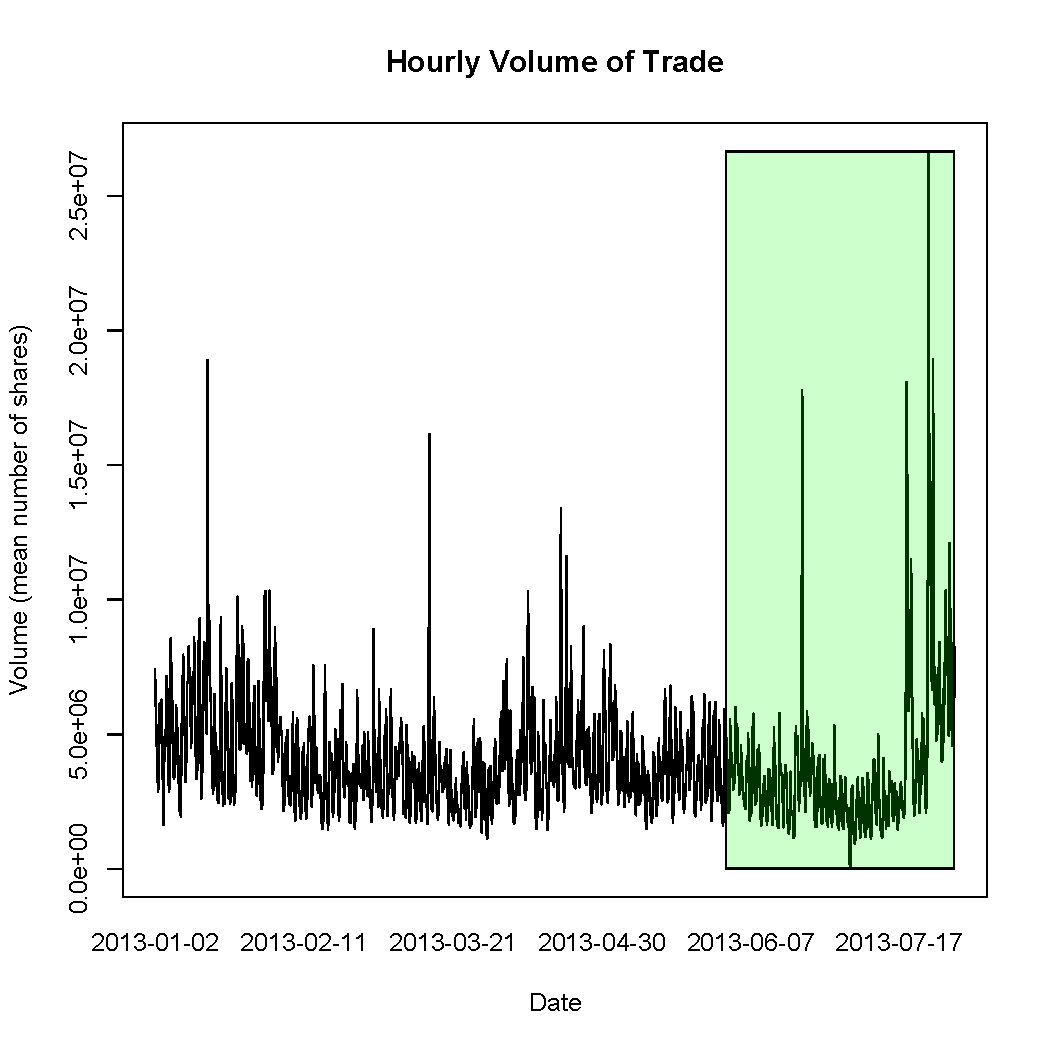
\includegraphics[scale=0.7]{june_july_volume.pdf} \\

\newpage

Let's start by taking a look at June in particular, we notice that somewhere around June 20th has large spike in volume. Below is a plot of June voume (black) and volatility (red) - clearly there's a large correlation between the two. This confirms our hypothesis that June 20th may have been very important for the market - at least in the ultra short horizon of a day or two in June. \\

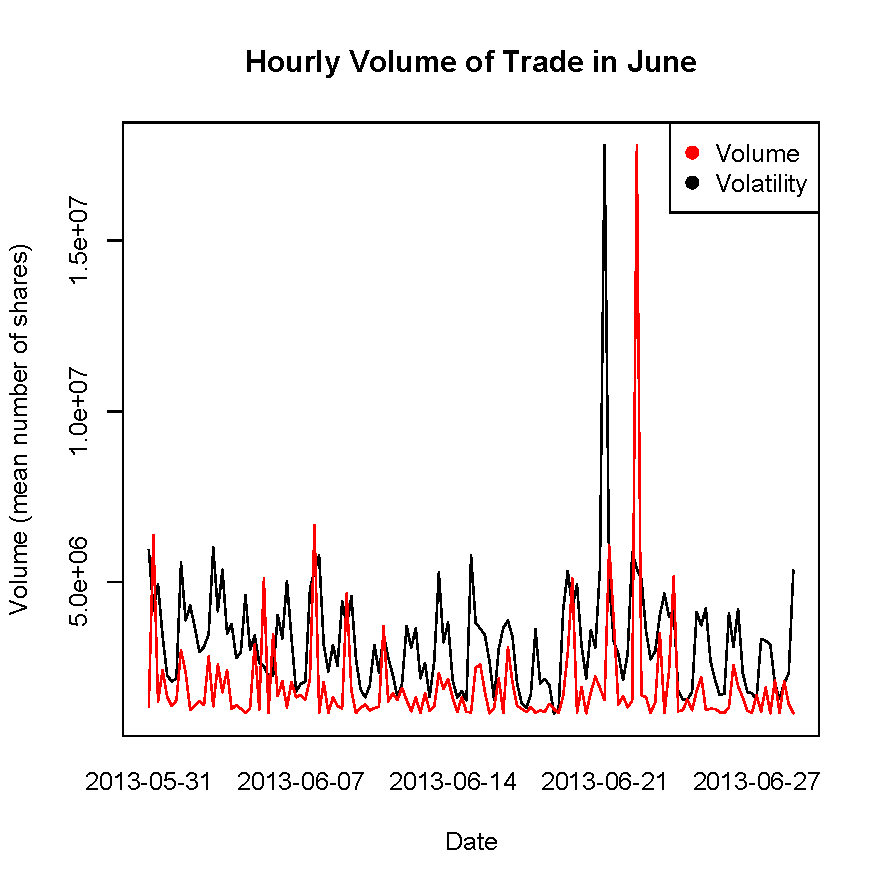
\includegraphics[scale=0.5]{june_volume_volatility.pdf} \\

\newpage

Now let's take a look at July. Overall, it looks like June 15th - 30th has a lot of volatiltiy in the volume. These results are similar to those we found for the volatility in the returns and are likely linked to the earnings reports for the respective companies, not an NSA leak. \\

In particular, Google and Microsft had their reports on the 18th, while Facebook and Apple had theirs on the 24th. \\

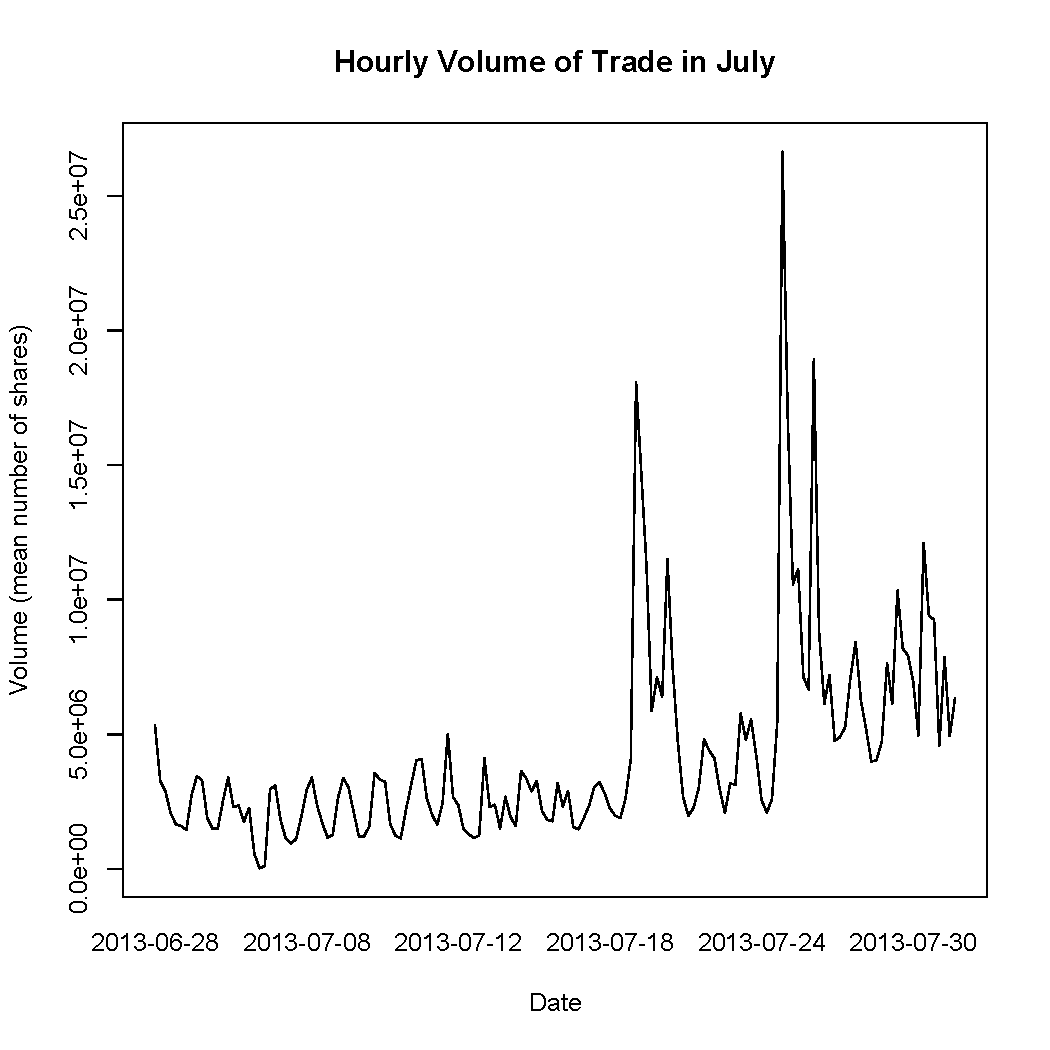
\includegraphics[scale = 0.5]{july_volume.pdf} \\

\end{document}